%%%%%%%%%%%%%%%%%%%%%%%%%%%%%%%%%%%%%%%%%%%%%%%%%%%%%%%%%%%%%%%%%
%%% Praca inżynierska -- Maciej Pereślucha
%%% Oparta na szablonie pracy dyplomowej WEII PRz (styczeń 2024)
%%% Oryginał szablonu z instrukcjami formatowania:
%%% https://github.com/przemarbor/szablon_pracy_dyplomowej_weii
%%%%%%%%%%%%%%%%%%%%%%%%%%%%%%%%%%%%%%%%%%%%%%%%%%%%%%%%%%%%%%%%%

\documentclass[12pt, twoside, openright]{article}

\usepackage{weiiszablon}
\usepackage[section]{placeins}

\author{Maciej Pereślucha}
\studentID{EF-177139}

\title{Zastosowanie algorytmów sztucznej inteligencji do rozpoznawania autentyczności podpisu}
\titleEN{Application of Artificial Intelligence Algorithms for Signature Authenticity Recognition}

% 1 = inżynierska, 2 = magisterska, 3 = doktorska
\newcommand{\rodzajPracyNo}{1}

\supervisor{dr inż. Paweł Górka}
\supervisorEN{Paweł Górka, PhD, Eng.}

% TODO: uzupełnić na końcu pisania pracy
\abstract{Treść streszczenia po polsku}
\abstractEN{Treść streszczenia po angielsku}
\keywords{max. 5 słów kluczowych w 2 wierszach, oddzielanych przecinkami}
\keywordsEN{max. five keywords in English}


\begin{document}

\maketitle
\cleardoublepage

\tableofcontents
\cleardoublepage


% TODO: odkomentować, gdy w tekście pojawią się skróty/symbole (np. CNN, EER, FAR, FRR)
% \section*{Wykaz symboli, oznaczeń i skrótów}
% \addcontentsline{toc}{section}{Wykaz symboli, oznaczeń i skrótów}


%%%%%%%%%%%%%%%%%%%%%%%%%%%%%%%%%%%%%%%%%%%%%%%%%%%%%%%%%%%%%%%%%
\section{Wprowadzenie}
\label{Sec:wprowadzenie}

Podpis odręczny jest jednym z~najczęściej używanych sposobów potwierdzania tożsamości, na przykład w~bankach, u~notariusza czy w~urzędach.
Sprawdzaniem, czy podpis jest prawdziwy, zajmują się zwykle biegli grafolodzy, jednak taka ocena zajmuje dużo czasu i~w~pewnym stopniu zależy od doświadczenia osoby, która ją wykonuje.
Automatyczna weryfikacja podpisu jest badana od kilkudziesięciu lat, ale nadal pozostaje problemem otwartym \cite{hafemann2017review}.
Rozwój uczenia głębokiego sprawił, że sieci neuronowe potrafią same nauczyć się cech, po których można odróżnić podpisy różnych osób, bez ręcznego projektowania tych cech.

Najprostszym pomysłem byłoby nauczenie sieci rozpoznawania podpisów każdej osoby osobno, tak jak w~zwykłym zadaniu klasyfikacji.
Takie podejście ma jednak dwie wady.
Po pierwsze, od jednej osoby dostępnych jest zwykle niewiele podpisów --- w~zbiorze użytym w~tej pracy są to 24 podpisy na osobę.
Po drugie, dodanie do systemu każdej nowej osoby wymagałoby ponownego trenowania modelu.
Rozwiązaniem jest sieć syjamska, która składa się z~dwóch jednakowych podsieci i~zamiast odpowiadać na pytanie, do kogo należy podpis, porównuje ze sobą dwa podpisy i~mierzy, jak bardzo są do siebie podobne \cite{bromley1993}.
Dzięki temu sieć może być stosowana także do osób, których podpisów nie widziała podczas treningu \cite{dey2017}.

W~pracy wykorzystano podpisy w~postaci zeskanowanych obrazów.
Taki wariant nazywa się weryfikacją statyczną (ang. \textit{offline}), w~odróżnieniu od weryfikacji dynamicznej (ang. \textit{online}), w~której podpis składany jest na tablecie rejestrującym na przykład prędkość ruchu pióra.
Na obrazie tych informacji nie ma, widoczny jest tylko kształt podpisu.
Najtrudniejsze do wykrycia są fałszerstwa wykwalifikowane, czyli podpisy podrobione przez osobę, która wcześniej ćwiczyła naśladowanie oryginału \cite{kalera2004}.
Wstępna analiza danych wykonana w~ramach pracy pokazała, że proste porównanie obrazów piksel po pikselu daje dla takich fałszerstw praktycznie ten sam wynik co dla dwóch prawdziwych podpisów tej samej osoby, dlatego potrzebna jest bardziej zaawansowana metoda.

Celem pracy było opracowanie systemu, który na podstawie zeskanowanego obrazu sprawdza, czy podpis jest autentyczny, oraz ocena jego skuteczności.
System oparto na sieci syjamskiej i~zaprojektowano tak, aby działał również dla osób, których podpisy nie były używane podczas treningu.
Zakres pracy obejmował:
\begin{itemize}[label={--},leftmargin=1.25cm]
	\item przegląd literatury dotyczącej weryfikacji podpisu i~sieci syjamskich,
	\item analizę zbioru podpisów CEDAR,
	\item przygotowanie danych, w~tym podział osób na osobne zbiory treningowy, walidacyjny i~testowy oraz utworzenie par podpisów,
	\item implementację sieci syjamskiej w~języku Python,
	\item trening sieci i~ocenę jej skuteczności na zbiorze testowym,
	\item analizę otrzymanych wyników.
\end{itemize}


%%%%%%%%%%%%%%%%%%%%%%%%%%%%%%%%%%%%%%%%%%%%%%%%%%%%%%%%%%%%%%%%%
% Tytuły rozdziałów 2--6 są robocze -- do uzgodnienia z promotorem
%%%%%%%%%%%%%%%%%%%%%%%%%%%%%%%%%%%%%%%%%%%%%%%%%%%%%%%%%%%%%%%%%
\section{Metody weryfikacji podpisu -- przegląd literatury}
\label{Sec:literatura}

% TODO: problem weryfikacji (online/offline, rodzaje fałszerstw), sieci syjamskie,
% funkcja straty kontrastowej, SigNet, miary oceny (FAR, FRR, EER)


\section{Zbiór danych i jego przygotowanie}
\label{Sec:dane}

\subsection{Zbiór CEDAR}
\label{Subsec:cedar}

Do trenowania i~testowania modelu wykorzystano zbiór podpisów CEDAR, przygotowany w~ośrodku Center of Excellence for Document Analysis and Recognition Uniwersytetu w~Buffalo.
Zbiór zawiera podpisy 55 osób, z~których każda złożyła 24 podpisy prawdziwe w~wyznaczonym polu o~wymiarach 2~$\times$~2 cale.
Fałszerstwa przygotowało około 20 innych osób, które miały jak najdokładniej podrobić podpisy osób ze zbioru, dzięki czemu dla każdej osoby zebrano 24 fałszerstwa wykwalifikowane.
Podpisy zeskanowano z~rozdzielczością 300 dpi w~8-bitowej skali szarości i~zapisano w~formacie PNG \cite{kalera2004}.
Podstawowe parametry zbioru zestawiono w~tabeli \ref{Tab:cedar}.

\begin{table}[ht]
\caption{Podstawowe parametry zbioru CEDAR}
\centering
	\begin{tabular}{|l|c|}
		\hline
		Parametr & Wartość \\
		\hline
		liczba osób & 55 \\
		podpisy prawdziwe na osobę & 24 \\
		fałszerstwa wykwalifikowane na osobę & 24 \\
		podpisy prawdziwe łącznie & 1320 \\
		fałszerstwa łącznie & 1320 \\
		wszystkie obrazy & 2640 \\
		\hline
	\end{tabular}
\label{Tab:cedar}
\end{table}

Zbiór CEDAR jest często wykorzystywany w~pracach dotyczących weryfikacji podpisu, między innymi w~\cite{dey2017,hafemann2017features}, dzięki czemu wyniki uzyskane w~niniejszej pracy można porównać z~wynikami innych autorów.

W~pracy użyto kopii zbioru udostępnionej w~serwisie Kaggle \cite{cedarkaggle}.
Obrazy podzielone są na dwa katalogi: \texttt{full\_org} z~podpisami prawdziwymi oraz \texttt{full\_forg} z~fałszerstwami.
Nazwa pliku zawiera numer osoby i~numer podpisu, na przykład \texttt{original\_1\_5.png} to piąty prawdziwy podpis osoby nr~1, a~\texttt{forgeries\_1\_5.png} to piąte fałszerstwo jej podpisu.
Według autorów zbioru wszystkie obrazy zapisano w~skali szarości, jednak w~użytej kopii część plików ma inne tryby kolorów, co opisano w~podrozdziale \ref{Subsec:eksploracja}.
Na rys. \ref{Fig:cedar_przyklad} przedstawiono przykładowe podpisy jednej osoby ze zbioru.

\begin{figure}[ht]
	\centering
	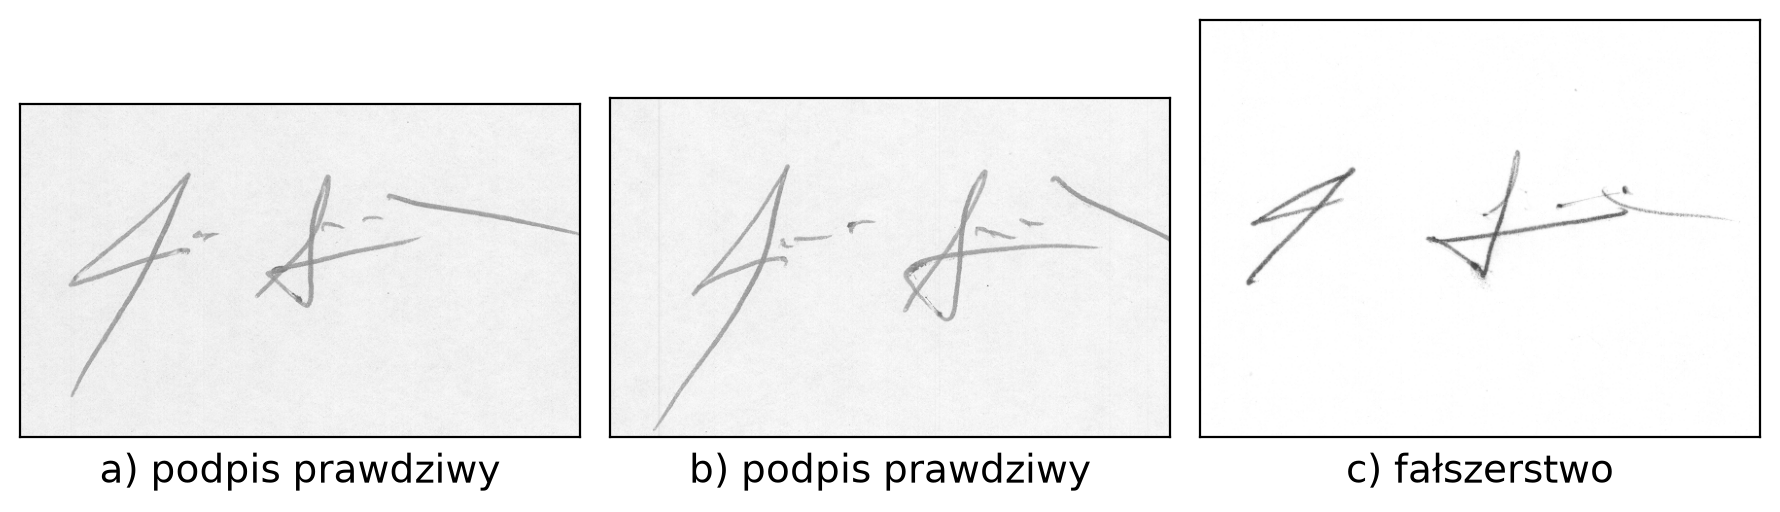
\includegraphics[width=\textwidth]{figures/cedar_przyklad.png}
	\caption{Przykładowe podpisy jednej osoby ze zbioru CEDAR: dwa podpisy prawdziwe (a, b) i~fałszerstwo wykwalifikowane (c)}
	\label{Fig:cedar_przyklad}
\end{figure}

\FloatBarrier
\subsection{Analiza eksploracyjna danych}
\label{Subsec:eksploracja}

Przed przygotowaniem danych do treningu przeprowadzono analizę zbioru, aby sprawdzić jego poprawność i~wykryć cechy obrazów, które mogłyby utrudnić trening sieci albo zafałszować wyniki.
Analizę wykonano w~języku Python z~użyciem bibliotek PIL i~NumPy.

Najpierw sprawdzono kompletność zbioru.
W~katalogu \texttt{full\_org} znajduje się 1320 obrazów i~tyle samo w~katalogu \texttt{full\_forg}, po 24 dla każdej z~55 osób.
Dla każdego pliku obliczono skrót MD5, co pozwoliło stwierdzić, że w~zbiorze nie ma powtórzonych obrazów.
Sprawdzono także, czy wszystkie pliki dają się poprawnie otworzyć, i~żaden nie okazał się uszkodzony.
Oprócz obrazów w~katalogach znajdują się jedynie pliki systemowe \texttt{Thumbs.db}, które pominięto.

Następnie sprawdzono tryby kolorów obrazów.
Według autorów zbioru wszystkie podpisy zapisano w~8-bitowej skali szarości \cite{kalera2004}, jednak w~użytej kopii podpisy prawdziwe zapisane są w~trybach RGBA (cztery kanały) i~L (skala szarości), a~fałszerstwa w~trybach P (paleta kolorów) i~RGBA.
Kolor nie niesie informacji o~kształcie podpisu, dlatego wszystkie obrazy przy wczytywaniu zamieniane są na skalę szarości.

Obrazy w~zbiorze nie mają wspólnego rozmiaru.
Wśród 1320 podpisów prawdziwych występuje 1095 różnych rozmiarów, a~wśród fałszerstw 1006.
Mediana rozmiaru wynosi 576~$\times$~349 pikseli (szerokość $\times$ wysokość), a~szerokość obrazów waha się od 264 do 888 pikseli.
Sieć wymaga obrazów o~jednakowym rozmiarze, dlatego wszystkie obrazy trzeba przeskalować.
Ponieważ podpisy są wyraźnie szersze niż wyższe (proporcja około 1,65:1), wejście sieci powinno mieć kształt prostokąta, a~nie kwadratu.
Okazało się również, że rozmiar obrazu niemal jednoznacznie wskazuje osobę, do której należy podpis: 85,4\% rozmiarów występujących wśród podpisów prawdziwych i~78,1\% wśród fałszerstw pojawia się tylko u~jednej osoby.
Gdyby obrazy nie zostały ujednolicone, sieć mogłaby nauczyć się rozpoznawać osobę po rozmiarze obrazu, a~nie po kształcie podpisu.

Sam podpis zajmuje średnio około 60\% powierzchni obrazu (60,1\% dla podpisów prawdziwych i~58,6\% dla fałszerstw), a~resztę stanowi puste tło.
Wartości te obliczono jako stosunek pola prostokąta obejmującego podpis do pola całego obrazu, przy czym za piksele podpisu uznano piksele o~jasności mniejszej niż 200.
Przeskalowanie całego obrazu do niewielkiego wejścia sieci oznaczałoby, że znaczna jego część przypadałaby na tło, dlatego przed skalowaniem obrazy przycinane są do prostokąta zawierającego podpis.

Najważniejszym wynikiem analizy okazała się różnica w~jasności tła między podpisami prawdziwymi a~fałszerstwami.
Dla każdego obrazu obliczono medianę jasności pikseli, która, ponieważ podpis zajmuje tylko niewielką część pikseli, odpowiada w~przybliżeniu jasności tła.
Rozkład tej wartości przedstawiono na rys.~\ref{Fig:tlo_histogram}.

\begin{figure}[ht]
	\centering
	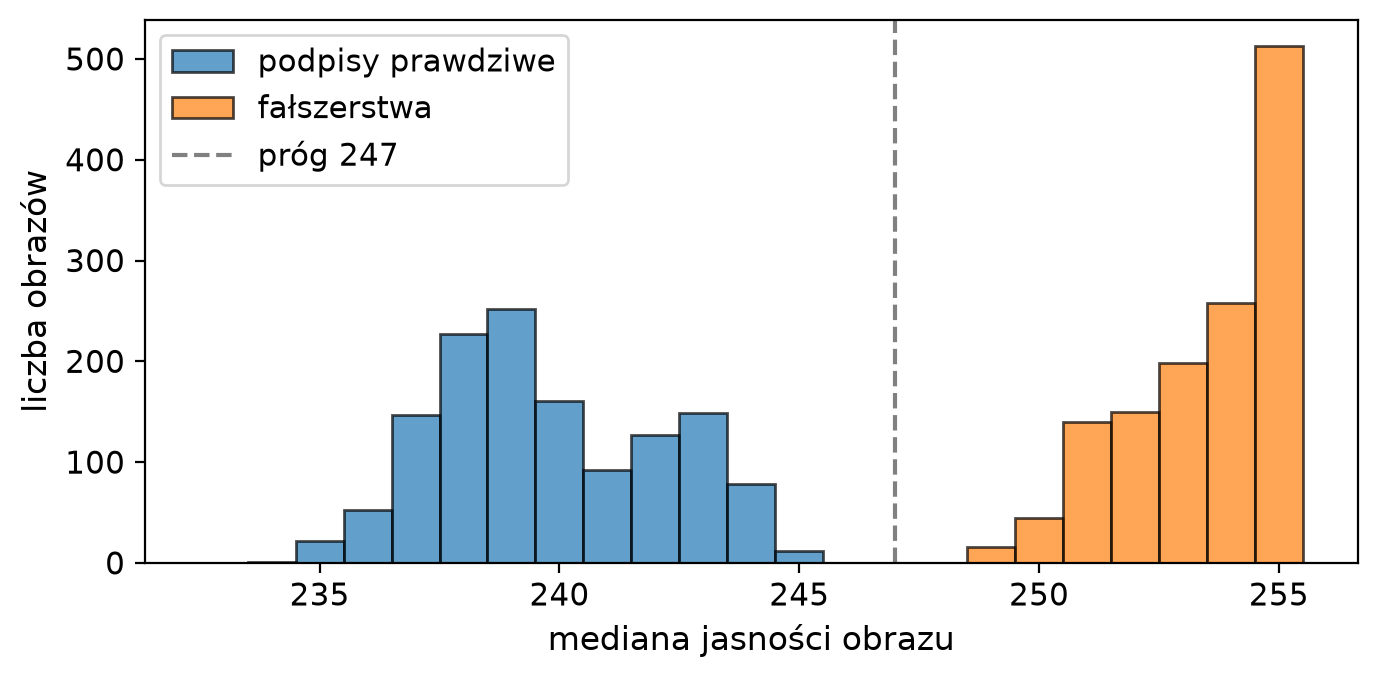
\includegraphics[width=0.8\textwidth]{figures/tlo_histogram.png}
	\caption{Rozkład mediany jasności obrazów dla podpisów prawdziwych i~fałszerstw w~zbiorze CEDAR}
	\label{Fig:tlo_histogram}
\end{figure}

Dla podpisów prawdziwych mediana mieści się w~przedziale od 234 do 245 (średnio 239,8), a~dla fałszerstw od 249 do 255 (średnio 253,5), przy czym 513 z~1320 fałszerstw ma tło idealnie białe.
Przedziały te nie nakładają się, więc pojedynczy próg jasności równy 247 pozwala bezbłędnie oddzielić wszystkie podpisy prawdziwe od fałszerstw bez analizowania samego podpisu.
Sieć trenowana na takich danych mogłaby wykorzystać tę różnicę zamiast uczyć się cech podpisu, co zawyżyłoby wyniki dla fałszerstw wykwalifikowanych.
Na podstawie dostępnych informacji nie da się ustalić, czy różnica ta pochodzi z~oryginalnego skanowania, czy z~późniejszej konwersji plików.
Sposób jej usunięcia opisano w~rozdziale~\ref{Sec:model}.

Na koniec sprawdzono, czy do odróżniania podpisów wystarczy proste porównanie obrazów.
Obrazy przeskalowano do rozmiaru 128~$\times$~128 pikseli i~dla par obrazów obliczono współczynnik korelacji Pearsona między wartościami pikseli.
Średnia korelacja dla par dwóch podpisów prawdziwych tej samej osoby wyniosła 0,146, dla par złożonych z~podpisu prawdziwego i~fałszerstwa tej samej osoby również 0,146, a~dla par podpisów dwóch różnych osób 0,081.
Taka metoda odróżnia więc podpisy różnych osób, ale nie odróżnia fałszerstw wykwalifikowanych od podpisów prawdziwych, co uzasadnia zastosowanie sieci neuronowej.

\subsection{Podział na zbiory niezależne od autora}
\label{Subsec:podzial}

\subsection{Budowa par podpisów}
\label{Subsec:pary}


\section{Model sieci syjamskiej}
\label{Sec:model}


\section{Badania eksperymentalne i wyniki}
\label{Sec:wyniki}


\section{Podsumowanie i wnioski końcowe}
\label{Sec:podsumowanie}

% TODO: ostatni akapit musi zaczynać się od: ,,Autor za własny wkład pracy uważa: \ldots''


%%%%%%%%%%%%%%%%%%%%%%%%%%%%%%%%%%%%%%%%%%%%%%%%%%%%%%%%%%%%%%%%%
% TODO: odkomentować, jeśli będą załączniki (np. instrukcja uruchomienia kodu)
% \section*{Załączniki}
% \addcontentsline{toc}{section}{Załączniki}


\clearpage
\addcontentsline{toc}{section}{Literatura}

% Kolejność pozycji = kolejność pierwszego \cite w tekście
\begin{thebibliography}{9}
\bibitem{hafemann2017review} Hafemann L.G., Sabourin R., Oliveira L.S.: Offline Handwritten Signature Verification --- Literature Review. 7th International Conference on Image Processing Theory, Tools and Applications (IPTA), 2017.
\bibitem{bromley1993} Bromley J., Guyon I., LeCun Y., Säckinger E., Shah R.: Signature Verification using a ,,Siamese'' Time Delay Neural Network. Advances in Neural Information Processing Systems 6 (NIPS 1993), str. 737--744.
\bibitem{dey2017} Dey S., Dutta A., Toledo J.I., Ghosh S.K., Lladós J., Pal U.: SigNet: Convolutional Siamese Network for Writer Independent Offline Signature Verification. arXiv:1707.02131, 2017.
\bibitem{kalera2004} Kalera M.K., Srihari S.N., Xu A.: Offline Signature Verification and Identification Using Distance Statistics. International Journal of Pattern Recognition and Artificial Intelligence, vol.~18, nr~7, 2004, str. 1339--1360.\bibitem{hafemann2017features} Hafemann L.G., Sabourin R., Oliveira L.S.: Learning Features for Offline Handwritten Signature Verification using Deep Convolutional Neural Networks. Pattern Recognition, vol.~70, 2017, str. 163--176.
\bibitem{cedarkaggle} CEDAR Signature Dataset, \url{https://www.kaggle.com/datasets/shreelakshmigp/cedardataset}. Dostęp 29.09.2026.

\end{thebibliography}

\clearpage
\makesummary

\end{document}